%=== CHAPTER THREE (3) ===
%=== (Actual work done and contribution, including literature survey) ===

\chapter{RVPG: Refined VP Guided Lane Detection}
\label{cha:model}
\begin{spacing}{1.5}
\setlength{\parskip}{0.3in}
%  (Actual work done and contribution, including literature survey)

The next few chapters should describe the work you have done in tackling the problem. There might be a chapter on the fundamental theories relevant to the solution you are pursuing, or the supporting technologies you need in implementing the solution. Then there should be a chapter on the solution itself, followed by a chapter on the results and analysis of the results.

\section{Introduction}

say something why its strange

\section{Improved Vanishing Point Directed Neural Network}
\label{sec:MD_model}

\subsection{Overview}
The network in my work is called \textbf{RVPG Net (Refined Vanishing Point Guided Network)}. It was developed based on the VPGNet~\cite{lee2017vpgnet} and has several improvements. The network aims at detecting and classify the lanes and the road markings simultaneously, on the pixel-level. The lanes are predicted with on the guide of vanishing point. 

Multi-task combined with Convolutional Neural Network is a solid solution in traffic-sign prediction. In a research about traffic-sign design in 2016~\cite{zhu2016traffic, huval2015empirical}, researchers proposed a deep Convolutional Neural Network (CNN) structure to detect and classification those small-scaled road markings. Besides, they proposed a benchmark containing a variety of traffic signs and road markings. Because this network is good at small object detection, it can extracts the high-level features from the image, thus are more resistant to the distortion in a small area. This stability can be extended to application in rainy conditions, that the rain drop's negative effects will be offset. Based on their work, RVPG net also uses the CNN structure and multi-task method to resist the distortion of rain drop and bad illumination.

Vanishing point can direct the prediction of the curved roads. Vanishing point is the visual intersection of two parallel lines, in our case the vanishing point is the end of two converging lanes, as shown in TBC. This Vanishing Point information is utilized by human eyes, usually unconsciously, to guess the trend of the curved road. By this mechanism, human is able to predict the tendency for a long distance rather than focus only on the short distance in front of the car.

The main feature of the RVPG is the multi-task and the VP feeding. With these two design of structure, the RVPG can extract the features from the original image significantly, and it shows high accuracy \& F1-Score in the detection and classification of road markings.

\subsection{Architecture}

The architecture of the RVPG is shown in \autoref{fig:structure}. It mainly consists three stages:

\begin{enumerate} \vspace{-5mm}
    \item The convolution layers stack
    \item The multi-branch
    \item The feature combination layers stack
\end{enumerate} \vspace{-5mm}

\begin{figure}[ht]
\centering
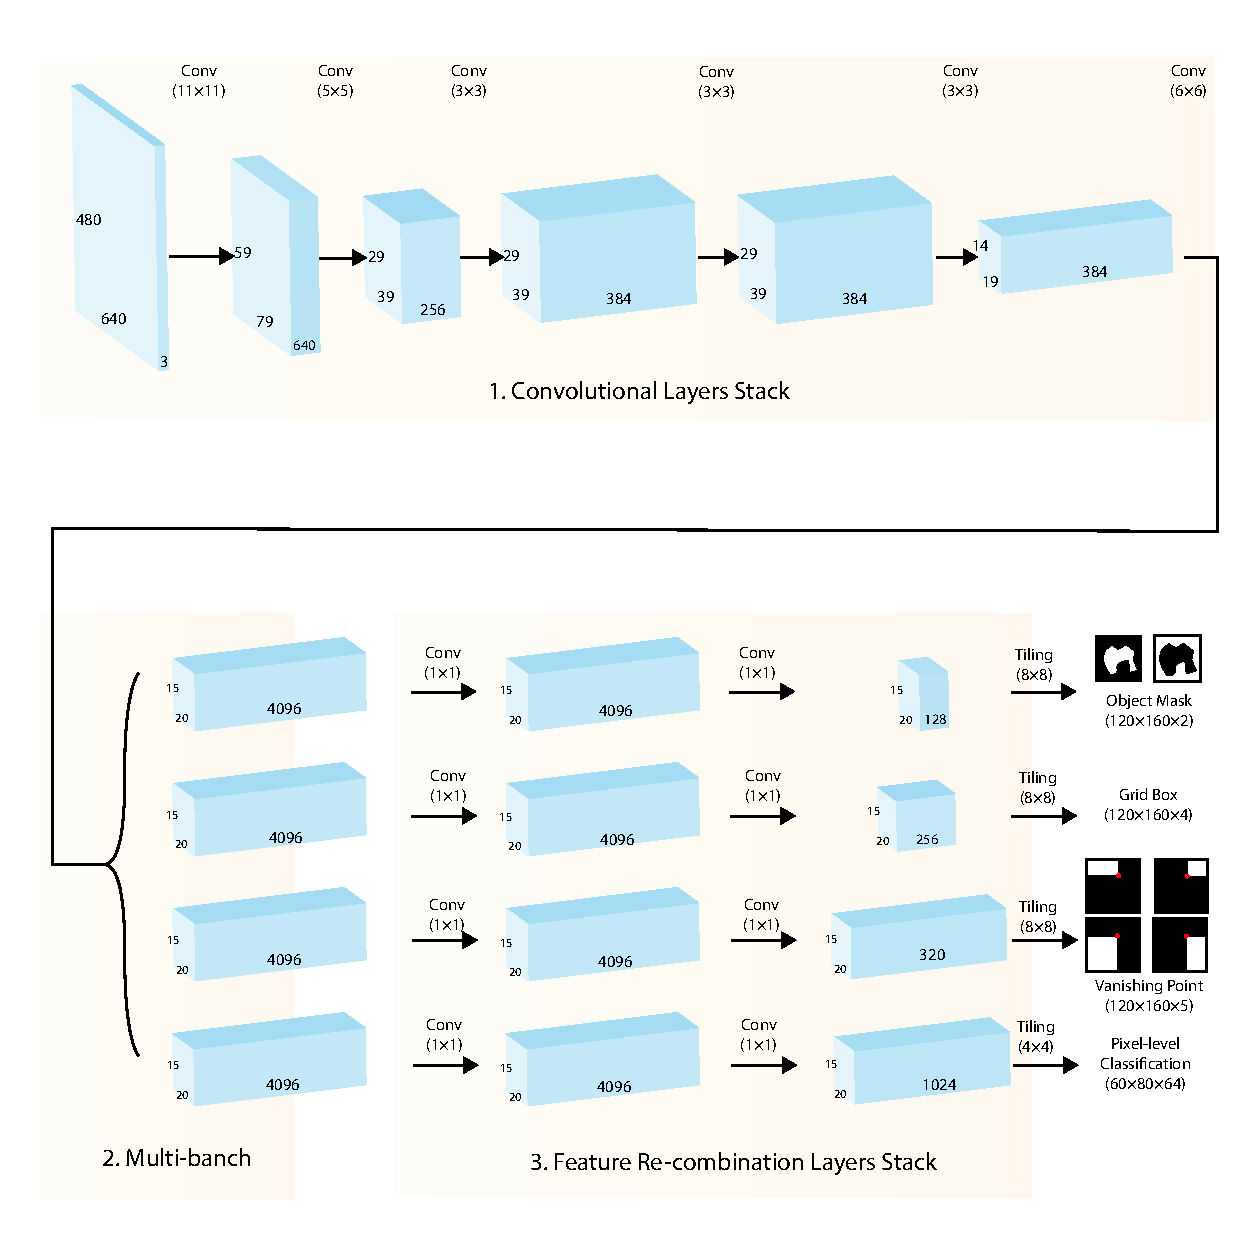
\includegraphics[width=0.99\textwidth, fbox]{Chapter3/structure.pdf}
\caption{the Structure of RVPG Network}
\label{fig:structure} 
\end{figure}

The first stage is a convolutional layer stack structure, it is aimed at extracting features. The input image is of size $480 \times 640 \times 3$\footnote{Because the relative fixde structure of network, in RVPG only 480*640 can be accepted as input. However, do re-design on network convolutional layer configuration will fit to any other size.}, in which $3$ is the RGB three color channel. Just like the CNN, the first stage of RVPG use different sizes of $2-D$ convolutional kernel to convolve the input image. In RSVP, I use the ReLU (Rectified Linear Unit, shown in \autoref{fig:relufunc}) activation function to do non-linear mapping in neutron, and the max-pooling layer to reduce the feature maps size. The target of this fist stage is to extract higher dimension of feature maps. For example, the first convolution layers' output represents the existence of the continuous edges around the object; the second convolution layers' output represents the relative position between those extracted edge features; the third convolution layers' output represents the group information of edges that are non-intersected; and so on... With deeper of the convolutional operation go, the more abstract the feature extracted are. In RVPG, five continuous convolutional layers are used in first stage.

The second stage is the multi-branch which will split the task into four different tasks simultaneously, the parameters behind the bifurcation would be shared by all tasks, but the parameters after the bifurcation would belong to each task separately. This design of multi-task have two advantages: 1) Let the different task share information. 2) Do multi-task prediction. This structure will be explained in \autoref{subsec:multitask}.

The third stage is the feature re-combination layers stack, which aims at the convergence of feature map depth towards output size. The structure in this stage is similar to CNN (As shown in lower half of \autoref{fig:structure}), but with very thick feature map layers. As can be seen, the feature map depth is $15 \times 20 \times 4096$, $15 \times 20 \times 4096$ and $15 \times 20 \times k$, in which $k \in \{128, 256, 320, 1024\}$ for different branches. Each of the convolutional layer is using $1 \times 1$ convolutional kernel. Here, the $1 \times 1$ convolutional kernel is a way to reduce out put dimension. As shown in \autoref{fig:oneonekernel}, if we want to reduce a feature map stack of size $W \times H \times N$, to $W \times H \times D, (D \neq N)$, just apply $D$ kernels of $1 \times 1 \times N$ size.

\begin{figure}[ht]
\centering
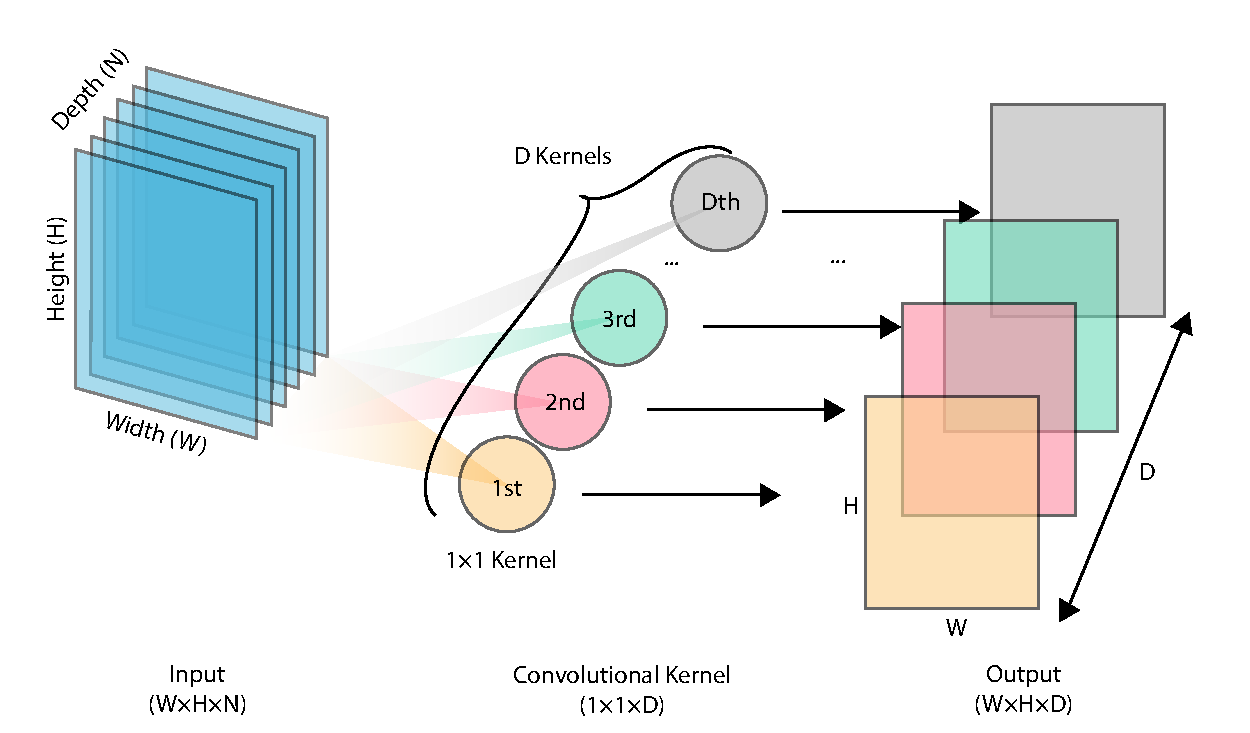
\includegraphics[width=0.99\textwidth, fbox]{Chapter3/oneonekernel.pdf} % TBC: Single kernel 1x1xN, all 1x1xNxD
\caption{Relationship between Size of Input, Kernel Num and Output}
\label{fig:oneonekernel} 
\end{figure}

The entire convolutional layers stack configuration and its index are shown in \autoref{tab:convlayer}.

\begin{table}[ht]
\centering
\caption{Convolutional Layers and Pooling Configuration}
\label{tab:convlayer}
\resizebox{\textwidth}{!}{%
\begin{tabular}{@{}ccccc@{}}
\toprule
Layer & (Kernel Size, Stride, Pad) & (Pooling Size, Stride) & Addition & Receptive Field \\ \midrule
Conv 1 & (11, 4, 0) & (3, 2) & LRN & 11 \\
Conv 2 & (5, 1, 2) & (3, 2) & LRN & 51 \\
Conv 3 & (3, 1, 1) & $-$ & $-$ & 99 \\
Conv 4 & (3, 1, 1) & $-$ & $-$ & 131 \\
Conv 5 & (3, 1, 1) & (3, 2) & $-$ & 163 \\
Conv 6 & (6, 1, 3) & $-$ & Dropout & 355 \\
Conv 7 & (1, 1, 0) & $-$ & Dropout & 355 \\
Conv 8 & (1, 1, 0) & $-$ & Branched & 355 \\ \bottomrule
\end{tabular}%
}
\end{table}

The combination of three stages can achieve four tasks at one prediction, besides, for each branch, the information learned from other branches maybe helpful to know the context of input images.

\subsection{Multi-task Structure}
\label{subsec:multitask}

Multi-task structure is the main highlight of the RVPG net. The training network are divided into four branches, each branch stands for one task in the lane and road marking, as shown in struacture diagram in \autoref{fig:structure}
% \vspace{-0mm}
\begin{align}
    F = \frac{P_{obj}}{H \times W} \times 100\% \label{eq:fore}
\end{align}
\vspace{-7mm}
\begin{equation}
    B = \frac{P_{bg}}{H \times W} \times 100\% \label{eq:bg}
\end{equation}

The first branch is the object mask task, basically a semantic detection of target object. Its output is of size $120 \times 160 \times 2$, containing 2 feature maps. In the $1$st feature map, the foreground pixels (detected objects) are set to be $1$, and other pixels are $0$. In the $2$nd feature map, the foreground pixels are set to be $0$, and the background is set to be $1$. This scheme is better than only using $1$ frame for background/foreground, because only detect the background or foreground maybe instability when either of them not easy to detect. By using both foreground and background, results can be combined for post-processing. For example, if using all-background, when the object is very small, the percentage of \autoref{eq:bg} will be very large, and the network will tend to predict all the pixels as background to achieve lower loss. In this situation, the foreground frame is very important. By using loss function like F1 score, even a small area in foreground will affect the result effectively. Thus, by combining the foreground and background 2 frames, the model will not converge at all-back or all-fore.

The second branch is the grid box branch, which is additional information for locating the objects, but finally proved to be useless. This branch is originated from VPGNet~\cite{lee2017vpgnet}. It just feeds low-definition grid boxes to the network, hopefully the network will learn to locate the object on a rough coordinate. The experimental results without this branch do not have much difference, thus we remove it in RVPG.

The third branch is Vanishing Point prediction task, in which the network will predict a $(X,Y)$ coordinate of Vanishing Point based on given image. This branch will output $120 \times 160 \times 5$ feature map. It uses $5$ channels, as 1) First channel is the VP foreground map; 2) Second channel has all pixels on the left upper corner to Vanishing point as $1$ and other pixels $0$; 3) Third channel has all pixels on the right upper corner to Vanishing point as $1$ and other pixels $0$; 4) Fourth channel has all pixels on the left lower corner to Vanishing point as $1$ and other pixels $0$; 4) Fifth channel has all pixels on the right lower corner to Vanishing point as $1$ and other pixels $0$. Details are described in \autoref{subsec:fourmap}

The fourth branch is pixel-wise classification task. For each class, the network will give a confidential value of each pixel belonging to this class. The output size is $60 \times 80 \times 64$, in which $64$ means it can predict maximum $64$ types of road markings and lanes. In the RVPG, we uses the VPG data set and Cordova data set, in which only $17$ of road markings (including lane type) types are annotated. The classes and its index are listed in \autoref{tab:classes}.

\section{Caffe Implementation}
\label{sec:MD_CAFFE}

As the original VPGNet author implements the network using CAFFE\footnote{\url{https://github.com/SeokjuLee/VPGNet}}, I also use CAFFE as my start point. But judge from the results, CAFFE is not suitable to conduct quick deep learning experiments, and I would recommend follower researchers not using CAFFE but start with PyTorch or Keras based on our code.


\subsection{Database and Extraction}

Two sets of labeled lane data are used: 1) Caltech~\cite{caltech} lanes database; 2) VPGNet~\cite{lee2017vpgnet} Lanes and road marking database. 

First and mainly used is the VPG database. In VPG database, the image are not labeled pixel-wise, but labeled with $8 \times 8$ pixels block, which complies with the output size $120 \times 160$, 

\begin{table}[ht]
\centering
\caption{Classes Specification and its Index}
\label{tab:classes}
\begin{tabular}{clcl}
\toprule
Index & Lane Type          & Index & Road Marking Type   \\ \midrule
0     & Background         & 9     & Stop Line           \\
1     & Lane Solid White   & 10    & Arrow Left          \\
2     & Lane Broken White  & 11    & Arrow Right         \\
3     & Lane Double White  & 12    & Arrow Go Straight   \\
4     & Lane Solid Yellow  & 13    & Arrow U Turn        \\
5     & Lane Broken Yellow & 14    & Speed Bump          \\
6     & Lane Double Yellow & 15    & Cross Walk          \\
7     & Lane Broken Blue   & 16    & Safety Zone         \\
8     & Lane Slow          & 17    & Other Road Markings \\ \bottomrule
\end{tabular}
\end{table}%

\subsection{Environment Configuration}

CAFFE version etc table

\subsection{Training Data Preprocessing}



\subsection{4-Map: Vanishing Point Feeding Scheme}
\label{subsec:fourmap}

Why use, how to, what achieved.

\section{PyTorch Implementation}
\label{sec:MD_PyTorch}

\subsection{Motivation}

The drawback is severe: 1) CAFFE needs C++ debugging, which takes long time to compile each time. As a large network like VPGNet, it usually takes more than $10$ mins per compilation. 2) CAFFE is not friendly in document support, and lacks the user-friendly API, thus you need to go into all the C++ underlying code before do any change, even the most basic layer definition change. 3) CAFFE's support of GPU and CUDA suite is out-of-date, thus sometimes with the newest computer with RTX 3080 GPU, you may even not able to call the GPU support with CAFFE.

In a conclusion, don't use CAFFE anymore.

\subsection{Data Format Conversion}

\subsection{4-Tilling: Redesigned Tilling Layer}



\section{Improvements}
\label{sec:MD_improvement}
\setlength{\parskip}{0.3in}

\subsection{2-D Gaussian}
\label{subsec:IM_2D}

\subsection{Res Blocks}
\label{subsec:IM_resblock}

\subsection{E-Net}
\label{subsec:IM_Enet}



\section{Concluding Remarks}




%=== END OF CHAPTER THREE ===
\end{spacing}
\newpage
